
\documentclass[12pt]{article}
\usepackage{graphics,amssymb,amsmath}

\usepackage[slovak]{babel}
\usepackage[utf8]{inputenc}
\usepackage[IL2]{fontenc}

\usepackage{multicol}
\usepackage{mathtools}

\pagestyle{empty}
\setlength\textwidth{170mm}
\setlength\textheight{265mm}
\addtolength\oddsidemargin{-20mm}
\addtolength\topmargin{-20mm}
\setlength{\parindent}{1pt}
\setlength{\parskip}{10pt}
\newcount\pocet
\pocet = 1
\def\pr{{\bf \the \pocet .\ \global\advance\pocet by 1}}

\newcommand{\g}{ \dots \dots \dots \dots \dots \ }
\newcommand{\gu}{ \dots \dots \ }
\newcommand{\gr}{\dotfill \ }

\begin{document}

\newenvironment{itemize*}
{\begin{itemize}
\setlength{\itemsep}{0pt}
\setlength{\parskip}{0pt}}
{\end{itemize}}

\newenvironment{enumerate*}
{\begin{enumerate}
\setlength{\itemsep}{0pt}
\setlength{\parskip}{0pt}}
{\end{enumerate}}


\phantom{a}

\centerline{\textbf{\Large Matematika I}}
\smallskip
\centerline{05. január 2020}
\centerline{9:00}
\vskip0.5cm

\centerline{\bf  Meno a priezvisko: \gr Podpis: \gr}
\vskip0.5cm
\centerline{\bf  Ročník: \gr študijný program: \gr}
\vskip0.5cm

\medskip

\pr (7b) Daná je všeobecná rovnica kužeľosečky $y^2-4x^2+8x-8y-4=0$.\\
\textbf{Doplňte}
\begin{enumerate}
\item[a)] (2b) Kanonická rovnica (rovnica v štandardnom tvare) kužeľosečky je \gr
\item[b)] (1b) Typ kužeľosečky je \gr
\item[c)] (3b) Napíšte súradnice
\begin{itemize}
\item[$c_1$)] stredu kužeľosečky: \gr
\item[$c_2$)] ohnísk kužeľosečky: \gr
\item[$c_3$)] vrcholov kužeľosečky: \gr
\end{itemize}
\item[d)] (1b) Znázornite kužeľosečku a v náčrte popíšte jej charakteristické prvky.
\end{enumerate}

\newpage

\pr (2b) Vyberte funkciu, ktorej definičný obor je znázornený na obrázku.

\begin{multicols}{2}
\noindent
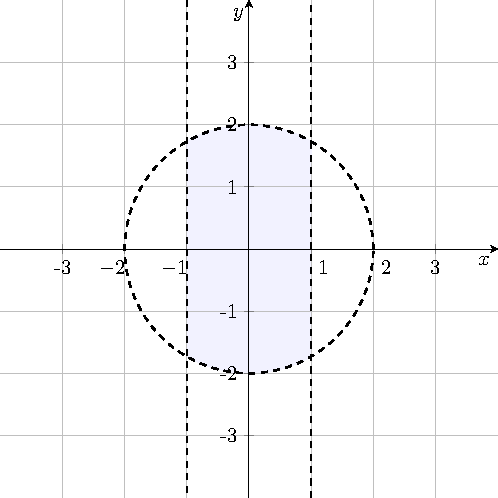
\includegraphics{kruznica1.pdf}

\noindent
\begin{itemize}
\item[a)] $\displaystyle f(x,y)= \ln\left(\frac{x+1}{x-1}\right)+\sqrt{4-x^2-y^2}$
\item[b)] $\displaystyle f(x,y)= \frac{\arcsin x}{\sqrt{4-x^2-y^2}}$
\item[c)] $\displaystyle f(x,y)= \frac{\ln(1-x^2)}{\sqrt{4-x^2-y^2}}$
\item[d)] $\displaystyle f(x,y)= \frac{\arcsin{(x+y)}}{\sqrt{4-x^2-y^2}}$
\end{itemize}
\end{multicols}

\pr (6b) Vypočítajte
$$\iint\limits_{M}{xy} \ \mathrm{d}x \mathrm{d}y,$$
kde množina $M$ je mnohouholník s vrcholmi
$A=[1, 0]$,
$B=[2, 0]$,
$C=[2, 2]$,
$D=[1, 3]$.

\begin{enumerate}
\item[]\textbf{Výsledok:}\gr
\end{enumerate}

\pr (4b) Bod $M$ má v pravouhlej súradnicovej sústave súradnice:  $M=[3,\sqrt{3}, 3]$.

\begin{enumerate}
\item[a)] (2b) Vyberte správnu odpoveď:\\
Súradnice bodu $M$ v cylindrickej súradnicovej sústave sú:


\noindent
\begin{itemize}
\begin{multicols}{2}
\item[a)]  $\displaystyle M=[2\sqrt{3}, \, -\frac{\pi}{6}, \, 3]$
\item[b)]  $\displaystyle M=[2\sqrt{3}, \, -\frac{\pi}{3},  \, 3]$

\item[c)]  $\displaystyle M=[2\sqrt{3}, \, \frac{\pi}{3},  \, 3]$
\item[d)]  $\displaystyle M=[2\sqrt{3}, \, \frac{\pi}{6},  \, 3]$
\end{multicols}
\end{itemize}


\item[b)] (2b) Znázornite tento bod $M$ v cylindrickej súradnicovej sústave.

\begin{enumerate}
\item[]\textbf{Náčrt:}
\end{enumerate}
\end{enumerate}

\newpage

\bigskip

\pr (8b) Daná je lineárna obyčajná diferenciálna rovnica (LODR)
$y^{\prime\prime}(x) +6y^{\prime}(x)+9y(x)= e^{-3x}$.

\begin{enumerate}
\item[a)](2b) Napíšte charakteristickú rovnicu k danej diferenciálnej rovnici.
\medskip

\textbf{Charakteristická rovnica je:} \gr

\item[b)] (2b) Nájdite fundamentálny systém riešení diferenciálnej rovnice s nulovou pravou stranou.

\medskip

\textbf{Fundamentálny systém riešení je} \gr

\item[b)] (2b) Nájdite partikulárne riešenie uvedenej nehomogénnej rovnice.

\medskip

\textbf{Partikulárne riešene je} \gr

\item[c)] (2b) Napíšte všeobecné riešenie danej lineárnej diferenciálnej rovnice.

\medskip

\textbf{Všeobecné riešenie danej LODR je} \gr
\end{enumerate}

\pr (4b)
Pomocou priamky $y=x$ a paraboly $y=x^2$ ukážte, že limita neexistuje

$$
\lim\limits_{
[x,y]\rightarrow [0,0]}
\frac{3x^2y}{x^4+y^2}.
$$

\begin{enumerate}
\item[]\textbf{Výsledok:}\gr
\end{enumerate}

\pr (6b) Nájdite rovnicu dotykovej roviny $\tau$ ku grafu funkcie
$\displaystyle f(x,y)=\sin\frac{x}{y}$ \\
\hspace*{1.4cm} v bode $T=\left[\pi,1, z_{0}\right]$.

\begin{enumerate}
\item[] (2b) Nájdite $z_0$ a  \textbf{uveďte súradnice dotykového bodu}: \gr
\item[] (4b) Všeobecná \textbf{rovnica} dotykovej roviny $\tau$ je:\gr
\end{enumerate}

\pr (6b) Daná je funkcia
$\displaystyle f(x,y)=\sqrt{4+x^2+y^2}$,
bod $\displaystyle A=[1, \,2 ]$
a vektor $\displaystyle \vec{l}=\left(-1, \, 2\right)$.

\begin{enumerate}
\item[a)] (3b) Nájdite gradient funkcie $f(x,y)$ v bode $A$.
\medskip

\textbf{Gradient} funkcie $f(x,y)$ v bode $A$ je \gr

\item[b)] (3b) Vypočítajte deriváciu funkcie $f(x,y)$ v bode $A$ v smere vektora $\vec{l}$.
\medskip

\textbf{Derivácia} funkcie $f(x,y)$ v bode $A$ v smere vektora $\vec{l}$ je \gr
\end{enumerate}

\newpage

\bigskip

\pr (9b) Toto je príklad typu E

text text text \\ \\


\end{document}